\section{Ereignisalgebra} \label{section-ereignisse}
Die Modellierung von Versuchsausgängen mit der Menge $\Omega$
allein ist nicht in der Lage, zusätzliche Eigenschaften eines
Versuchsausgangs wiederzugeben.
Sie muss daher um den Begriff des Ereignisses erweitert werden.

\subsection{Ereignisse}
Oft sind die einzelnen Versuchsausgänge nicht von Interesse.
Viele Würfelspiele mit zwei Würfeln haben besondere Regeln, wenn
der Spieler zwei gleiche Augenzahlen wirft, einen sogenannten {\em Pasch}.
Die Regeln sind unabhängig vom Wert, es zählt nur die Tatsache,
dass die beiden Augenzahlen gleich sind.
Das Ereignis ``Pasch'' ist eingetreten, wenn der Versuchsausgang, also das
Paar von Augenzahlen, in der Menge
\[
\def\e#1{\epsdice{#1}\,\epsdice{#1}}
P=\{
\e{1},
\e{2},
\e{3},
\e{4},
\e{5},
\e{6}
\}
\]
liegt.

Auch einzelne Messwerte sind oft nicht interessant.
Ein Überspannungsereignis tritt zum Beispiel ein, wenn die Spannung
einen Wert überschreitet, oder wenn das Elementarereignis, also der Messwert,
in der Menge
\[
U=
\{x\in\mathbb R\,|\, x > x_{\text{Limite}}\}
\]
liegt.

Solche zusammengesetzten Ereignisse sind also immer Teilmengen von $\Omega$.
Wir können dies als eine Definition des Begriffs des Ereignisses
verwenden.

\begin{definition}
Ist $\Omega$ eine Menge von Versuchsausgängen, dann heisst eine Teilmenge
$A\subset\Omega$ ein {\em Ereignis}.
Man sagt, das Ereignis $A$ ist {\em eingetreten}, wenn bei einer Durchführung des
Experimentes ein Versuchsausgang $\omega\in A$ aufgetreten ist.
\end{definition}

\begin{beispiel}
\begin{figure}
\centering
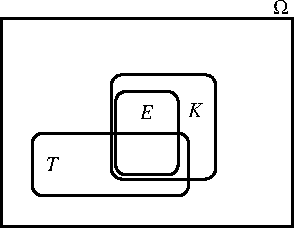
\includegraphics{images/ebola-1.pdf}
\caption{Ereignisse zum Experiment ``Person im Ebola-Gebiet''
\label{image-ebola}}
\end{figure}

In Abbildung~\ref{image-ebola} sind mögliche Ereignisse eines Experiments
dargestellt, bei dem ein zufällig ausgewählte Person daraufhin untersucht
wurde, ob sie mit Ebola in Kontakt kam, daran erkrankte und inzwischen
verstorben ist.
Der einzelne Versuchsausgang ist also die Person, die für die
Untersuchung ausgewählt wurde.
Die Menge $\Omega$ ist die Menge aller Personen.
Folgende Ereignisse wurden untersucht:
\begin{align*}
K&=\{\omega\in\Omega\,|\,\text{$\omega$ ist mit Ebola in Kontakt gekommen}\}
\\
E&=\{\omega\in\Omega\,|\,\text{$\omega$ ist an Ebola erkrankt}\}
\\
T&=\{\omega\in\Omega\,|\,\text{$\omega$ ist verstorben}\}
\end{align*}
Es gilt natürlich $E\subset K$, denn wer an Ebola erkrankt, muss mit
Ebola in Kontakt gekommen sein.
Das umgekehrte gilt nicht, man kann durchaus mit Ebola in Kontakt
kommen, ohne daran zu erkranken.

Es gilt nicht, dass $E\subset T$, denn einerseits gibt es Personen, die
Ebola überlebt haben, und andererseits gibt es an Ebola erkrankte,
die zur Zeit des Experiments noch nicht verstorben sind.
Die Menge $E\cap T$ besteht aus denjenigen Personen, die an Ebola
erkrankt waren und verstorben sind.
Dies heisst aber nicht, dass sie an Ebola gestorben sind.
\end{beispiel}

Zwei Ereignisse $A$ und $B$ können bei der Durchführung des Experimentes
gleichzeitig eintreten.
Der Versuchsausgang $\omega$ ist also so beschaffen, dass mit ihm sowohl
$A$ als auch $B$ eintreten, dass also $\omega\in A$ und $\omega\in B$,
oder $\omega \in A\cap B$.
Gleichzeitiges Eintreten von Ereignis $A$ {\em und} $B$ ist das Ereignis
$A\cap B$.

Tritt ein Ereignis $A$ bei einer Versuchsdurchführung nicht ein, dann trat
ein Versuchsausgang $\omega$ auf, der nicht zu $A$ gehört,
also $\omega\in\Omega\setminus A$.
Dies bedeutet aber, dass das Ereignis $\Omega\setminus A=\overline{A}$
eingetreten ist.
Nichteintreten des Ereignisses $A$ ist das Ereignis
$\overline{A}=\Omega\setminus A$.

Zwei Ereignisse sind speziell.
Die Menge $\Omega\subset\Omega$ hat die Eigenschaft, dass jeder denkbare
Versuchsausgang per Definition in $\Omega$ liegt, das Ereignis $\Omega$
tritt also immer ein.
$\Omega$ heisst daher auch das sichere Ereignis.
\index{Ereignis!sicheres}
Die leere Menge $\emptyset\subset\Omega$ hat genau die gegenteilige
Eigenschaft: was auch immer geschieht, was auch immer für ein 
Elementarereignis $\omega$ realisiert wird, in $\emptyset$ kann es
nicht drin sein, also wird $\emptyset$ nie eintreten.
$\emptyset$ heisst daher auch das unmögliche Ereignis.
\index{Ereignis!unmögliches}

Diese Beispiele zeigen, dass die Modellierung von Ereignissen als Teilmengen
von $\Omega$
mit der umgangssprachlichen Sprechweise von Ereignissen übereinstimmt.
Die Tabelle~\ref{begriffe-zusammenfassung}
fasst die gebräuchlichsten Mengenoperationen und die zugehörige
Sprechweise für Ereignisse zusammen.

\begin{table}
\begin{center}
\begin{tabular}{|l|c|}
\hline
Begriff&Modell\\
\hline
Elementarereignis&$\omega$\\
alle Elementarereignisse&$\Omega$\\
Ereignis&$A\subset\Omega$\\
sicheres Ereignis&$\Omega$\\
unmögliches Ereignis&$\emptyset$\\
$A$ und $B$&$A\cap B$\\
$A$ oder $B$&$A\cup B$\\
$A$ hat $B$ zur Folge, $A\Rightarrow B$&$A\subset B$\\
nicht $A$&$\Omega\setminus A$\\
\hline
\end{tabular}
\end{center}
\caption{Begriffe der Wahrscheinlichkeitstheorie und ihre mathematischen
Modellierung\label{begriffe-zusammenfassung}}
\end{table}

\subsection{Beispiele}
\subsubsection{AIDS-Test}
Wenn sich jemand im Bezug auf AIDS riskant verhalten hat, dann ist
eine seiner Sorgen, dass der AIDS-Test nicht sofort das richtige
Resultat anzeigt.
Und selbst wenn er die notwendige Frist abgewartet
hat, hat der Test eine geringe Fehlerrate.
Es können also verschiedene Ereignisse eintreten.
Meistens wird ein
positiver AIDS-Test richtig anzeigen, dass eine Person HIV hat.
Manchmal
wird der Test jedoch positiv sein, obwohl die Person gesund ist
und manchmal wird der Test zwar ein negatives Resultat zeigen,
aber die Person ist an HIV erkrankt.
Glück haben diejenigen, bei denen der Test nicht
anspricht, und die auch tatsächlich gesund sind.


\subsubsection{Euromillions}
\index{Euromillions}
\begin{figure}
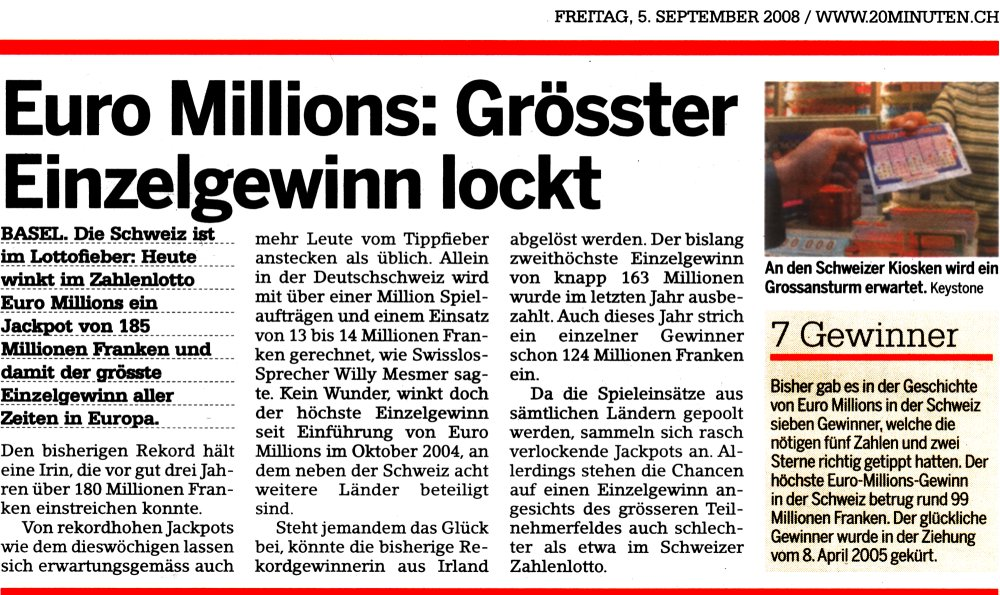
\includegraphics[width=\hsize]{graphics/euromillions}
\caption{Besondere Gewinnchance bei Euromillions}
\end{figure}
\begin{figure}
\begin{center}
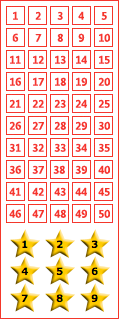
\includegraphics[height=8cm]{graphics/euromillionsschein}
\end{center}
\caption{Teilnahmeschein für Euromillions\label{euromillionsschein}}
\end{figure}
Am 5.~September 2008 schrieb die Gratiszeitung ``20 Minuten'', dass die
bevorstehende Ziehung der Lotterie Euromillions besondere Gewinnchancen 
ermögliche, weil der Jackpot ungewöhnlich gross sei.
Welche Ereignisse
sind in diesem Spiel relevant?

Auf der Euromillions-Website findet man die Erklärung, wie das Spiel abläuft.
Der Spieler kreuzt auf dem Teilnahmeschein (Abbildung~\ref{euromillionsschein})
fünf Zahlen und zwei Sterne an.
Dann erfolgt die Ziehung, Euromillions ermittelt
5 Gewinnzahlen aus dem Bereich 1--50 und 2 Gewinnsterne im Bereich 1--9.
Jetzt werden die Übereinstimmungen zwischen dem Tipp des Teilnehmers und den
Gewinnzahlen gezählt.
Je besser die Übereinstimmung desto grösser der Gewinn.

\begin{table}
\begin{center}
\begin{tabular}{|c|c|c|c|}
\hline
Gewinnrang&richtige Zahlen&richtige Sterne&Anteil Gewinnsumme\\
\hline
1&5&2&32.0\%\\
2&5&1&7.4\%\\
3&5&0&2.1\%\\
4&4&2&1.5\%\\
5&4&1&1.0\%\\
6&4&0&0.7\%\\
7&3&2&1.0\%\\
8&3&1&5.1\%\\
9&2&2&4.4\%\\
10&2&0&4.7\%\\
11&1&2&10.1\%\\
12&2&1&24.0\%\\
\hline
\end{tabular}
\end{center}
\caption{Gewinnränge bei Euromillions\label{gewinnraenge}}
\end{table}

Die Tabelle \ref{gewinnraenge} zeigt, wie der Gewinn verteilt wird.
Offenbar spielen dabei sogenannte Gewinnränge eine besondere Rolle.
Bei jedem Tippzettel wird festgestellt, in welchen Gewinnrang er
gehört.

Ausser den Gewinnrängen können auch andere Ereignisse eintreten,
die jedoch für die Auszahlung nicht unbedingt von Bedeutung sind,
oder aus denen sich der Gewinn noch nicht ableiten lässt:
\begin{itemize}
\item {\it Heiris Euromillions Teilnahmeschein fällt in Gewinnrang 10.}
Offenbar teilt sich Heiri 4.7\% der Gewinnsumme mit den anderen Teilnehmern,
die dasselbe Ergebnis erzielt haben.
\item {\it Hanna hatte fünf richtige Zahlen.}
Diese Information reicht noch nicht, um den Gewinn festzulegen.
Hannas Teilnahmeschein fällt in Gewinnrang 1 oder 2 oder 3.
\item {\it Hermine hatte keinen einzigen Stern richtig.}
Hermine könnte
etwas gewonnen haben, nämlich wenn sie 5, 4 oder 2 richtige Zahlen
gehabt hat (Ränge 3, 6 bzw.~10).
Oder sie könnte mit 3, 1 oder 0 richtigen Zahlen nichts gewonnen haben.
\item {\it Hermann hatte richtige Zahlen und Sterne.}
Hermann hatte also 1, 2, 3, 4 oder 5 richtige Zahlen {\em und}
1 oder 2 richtige Sterne.
\item {\it Es trifft nicht zu, dass Hilary einen richtigen Stern hat.}
\item {\it Holger hat auf 47 gesetzt.}
Dieses Ereignis nimmt auf die Ziehung überhaupt keinen Bezug,
trotzdem beschreibt es einen möglichen Ausgang des Experimentes.
\end{itemize}
Wir stellen fest, dass Ereignisse mit {\em und} (beide Ereignisse sind
eingetreten) und {\em oder} (eines der Ereignisse ist
eingetreten) verknüpft werden können.
Ausserdem können Ereignisse negiert werden.

\subsection{Produkte}
\begin{figure}
\begin{center}
\begin{tabular}{|c|c|c|c|c|c|}
\hline
(1,1)&(1,2)&(1,3)&(1,4)&(1,5)&(1,6)\\
\hline
(2,1)&(2,2)&(2,3)&(2,4)&(2,5)&(2,6)\\
\hline
(3,1)&(3,2)&(3,3)&(3,4)&(3,5)&(3,6)\\
\hline
(4,1)&(4,2)&(4,3)&(4,4)&(4,5)&(4,6)\\
\hline
(5,1)&(5,2)&(5,3)&(5,4)&(5,5)&(5,6)\\
\hline
(6,1)&(6,2)&(6,3)&(6,4)&(6,5)&(6,6)\\
\hline
\end{tabular}
\end{center}
\caption{Elementarereignisse für das Würfeln mit zwei unterscheidbaren
Würfeln\label{ereignisse-zwei-wuerfel}}
\end{figure}
Wir stellen uns vor, dass ein roter und ein blauer Würfel geworfen werden.
Die von den beiden Würfeln gezeigten Augenzahlen sind verschiedene
Versuchsausgänge, sozusagen ``rote'' und ``blaue'' Zahlen.
Das Resultat
eines Wurfes ist also ein Paar bestehend aus einer ``roten'' und
einer ``blauen'' Augenzahl.
Die Menge aller möglichen Ausgänge
ist also 
\[
\Omega = \Omega_{\text{rot}}\times\Omega_{\text{blau}},
\]
das kartesische Produkt der Mengen $\Omega_{\text{rot}}$ und
$\Omega_{\text{blau}}$ (siehe auch Abbildung \ref{ereignisse-zwei-wuerfel}).

In $\Omega$ lassen sich bereits bedeutend spannendere Ereignisse%
\footnote{\textit{Hinweis zu $A_2$}: $2|x \wedge 2|y$, sprich
	``2 teilt x und 2 teilt y'', ist äquivalent:
	$x \equiv 0 \imod{2} \wedge y \equiv 0 \imod{2}$
} beschreiben:
\begin{align*}
A_1&=\{\text{mindestens eine ungerade Zahl}\}\\
   &=\{(x,y)\in\Omega\;|\;x \equiv 1 \imod{2} \vee y\equiv 1 \imod{2}\},\\
A_2&=\{\text{beide Augenzahlen sind gerade}\}\\
   &=\{(x,y)\in\Omega\;|\;2|x \wedge 2|y\},\\
X_i&=\{(i,y)\in\Omega\},\\
Y_i&=\{(x,i)\in\Omega\},\\
S_s&=\{(x,y)\in\Omega\;|\; x + y = s\},\\
D_d&=\{(x,y)\in\Omega\;|\; |x - y| = d\}.
\end{align*}
Und damit lassen sich auch etwas spannendere Rechnungen durchführen.
Zum Beispiel:
\begin{align*}
A_1&=\Omega \setminus A_2 = \bar A_2,\\
A_1\cap A_2&=\emptyset,\\
A_1&=X_1\cup X_3 \cup X_5\cup Y_1\cup Y_3\cup Y_5,\\
X_4\cap Y_3&=\{(4,3)\},\\
X_5\cap S_7&=\{(5,2)\},\\
X_5\cap D_1&=\{(5,4), (5,6)\}.
\end{align*}
\begin{figure}
\centering
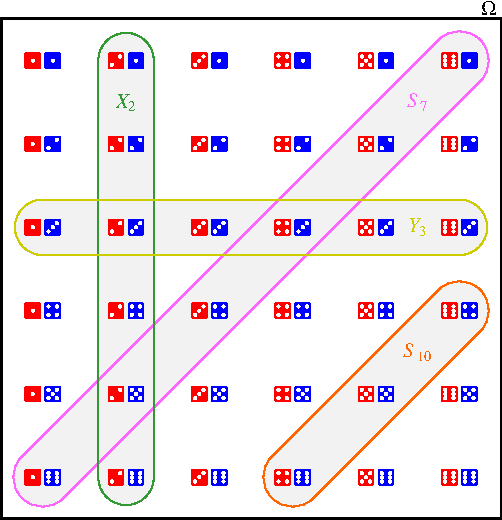
\includegraphics{images/zweiwuerfel-1.pdf}
\caption{Verschiedene Ereignisse in der Ereignisalgebra des Experiments
``Wurf zweier verschiedenfarbiger Würfel\label{zweiwuerfel}''}
\end{figure}

\subsection{Formale Definition}
Damit obige Definition von Ereignissen funktioniert, müssen
alle Operationen in der Tabelle~\ref{begriffe-zusammenfassung}
ausführbar sein.
Die Menge aller Teilmengen von $\Omega$, die Potenzmenge
$P(\Omega)$ erfüllt diese Bedingung,
ist aber sehr gross und hat sehr wenig nützliche Struktur, die
für den Aufbau des Begriffs der Wahrscheinlichkeit im nächsten
Abschnitt benötigt wird.
Insbesondere stellt sich heraus, dass es nicht möglich ist,
den Begriff der Wahrscheinlichkeit konsistent zu definieren, wenn
Ereignisse beliebige Teilmengen einer unendlichen Menge $\Omega$
sein dürfen.

Ein Beispiel für diese Situation sind Messwerte, in diesem
Fall ist $\Omega=\mathbb R$ unendlich.
Es werden aber auch nicht alle Teilmengen von $\mathbb R$ benötigt.
Es wird genügen, wenn wir alle Intervalle zur Verfügung haben sowie
alle Mengen, die sich daraus durch endlich viele Mengenoperationen
konstruieren lassen.
Statt der Menge $P(\Omega)$ wird also eine kleinere Menge $\cal A$
von Ereignissen verwendet.
Man kann zeigen, dass sich aus der Menge der Intervalle immer 
eine Menge von Ereignissen konstruieren lässt, in der alle
nötigen Operationen ausgeführt werden können, und auf der sich
die später einzuführende Wahrscheinlichkeit konsistent definieren
lässt.

Die Einschränkung auf $\cal A$ hat mindestens im Rahmen dieser
Vorlesung keine praktischen Konsequenzen, alle interessierenden
Ereignisse sind von vornherein in $\cal A$, und damit auch alle daraus
abgeleiteten Ereignisse.

Wir nennen eine solche Menge von Ereignissen eine Ereignisalgebra:

\begin{definition}
\label{def-ereignisalgebra}
Eine {\em Ereignisalgebra} $(\Omega,{\cal A})$ ist
eine Menge $\Omega$ mit einer Menge ${\cal A }\subset{\cal P}(\Omega)$
von Teilmengen von $\Omega$, die folgende Bedingungen erfüllen:
\begin{enumerate}
\item Vereinigungen von Elementen von ${\cal A}$ sind ebenfalls in ${\cal A}$,
also
\[
A,B\in {\cal A}\Rightarrow A\cup B\in{\cal A}
\]
\item Differenzen von Elementen von ${\cal A}$ sind in ${\cal A}$, also
\[
A,B\in {\cal A}\Rightarrow A\setminus B\in{\cal A}
\]
\item $\Omega\in{\cal A}$, d.~h.~es gibt das sichere Ereignis.
\end{enumerate}
\end{definition}

Sind nur die Bedingungen 1 und 2 erfüllt, spricht man auch von einem
Mengen-Ring.
Eine Ereignisalgebra heisst manchmal auch ein Mengenkörper.

Aus den Axiomen für die Ereignisalgebra lassen sich sofort erste
Schlussfolgerungen ziehen:
\begin{enumerate}
\item Es gibt auch das unmögliche Ereignis: $\emptyset = \Omega\setminus\Omega\in{\cal A}$.
\item Das Komplement eines Ereignisses ist ebenfalls ein Ereignis: $\bar A=\Omega\setminus A\in{\cal A}$.
\item Der Durchschnitt zweier Ereignisse ist ebenfalls ein Ereignis: $A\cap B = 
(A\cup B) \setminus ((A\setminus B) \cup (B\setminus A))\in{\cal A}$.
\end{enumerate}

